%%This is a very basic article template.
%%There is just one section and two subsections.
\documentclass{article}

%definitions for Formelsammlung

\usepackage[left=1.5cm,right=1.5cm,top=2.5cm,bottom=2cm,landscape]{geometry} 
\usepackage{multicol}
\usepackage[ngerman]{babel}
\usepackage{tabularx}
\usepackage{mathpazo}
\usepackage{mathtools}
\usepackage{amsmath}  
\usepackage{setspace} 
\usepackage{commath}
\usepackage[utf8]{inputenc}
%\usepackage[ansinew]{inputenc}  
\usepackage[T1]{fontenc}
\usepackage{lmodern} 
\usepackage{hyperref}
\usepackage{bigints}
\usepackage{array}
\usepackage[table]{xcolor}
\usepackage{layouts}
\usepackage{siunitx}
\usepackage{wrapfig}
\usepackage{multirow,bigstrut}
\usepackage{trfsigns}
\usepackage{amssymb} 
\usepackage{fancyhdr}
\usepackage{datetime}
\usepackage{pgfplots}
\usepgfplotslibrary{fillbetween}
\usepackage{listings}
\usepackage{mathrsfs}
\usepackage{tabu}
\usepackage{pdflscape}
\usepackage{booktabs}
%\usepackage{mathabx}
\usepackage{graphicx}
\usepackage{supertabular}
\usepackage{siunitx}
\usepackage[europeanvoltages, europeancurrents, europeanresistors, americaninductors, smartlabels]{circuitikz}

\DeclareMathOperator\arctanh{arctanh}
\DeclareMathOperator\arsinh{arsinh} 
\DeclareMathOperator\arcosh{arcosh}
\DeclareMathOperator\artanh{artanh}
\DeclareMathOperator\arcoth{arcoth} 
\DeclareMathOperator\sinc{sinc} 
\DeclareMathOperator\sgn{sgn} 
\DeclareMathOperator\LPF{LPF} 
\DeclareMathOperator\Q{Q} 
\DeclareMathOperator\erf{erf} 
\DeclareMathOperator\var{Var} 
\DeclareMathOperator\Cov{Cov} 
\DeclareMathOperator\floor{floor} 
\DeclareMathOperator\E{E} 
\DeclareMathOperator\NDFT{DFT} 
\DeclareMathOperator\IDFT{IDFT} 


%colorCodes
\definecolor{listinggray}{gray}{0.9}
\definecolor{lbcolor}{rgb}{0.95,0.95,0.95}
\definecolor{lightGray}{gray}{0.1}

\definecolor{cOrange}{HTML}{996633}
\definecolor{clOrange}{HTML}{DBB48D}
\definecolor{cBlue}{HTML}{336699}
\definecolor{clBlue}{HTML}{A0BCD8}
\definecolor{cGreen}{HTML}{339966}
\definecolor{clGreen}{HTML}{94D4B4}
\definecolor{cRed}{HTML}{993333}
\definecolor{clRed}{HTML}{D0B0B0}
\definecolor{cGray}{gray}{0.4}
\definecolor{clGray}{gray}{0.96}



\setlength{\parindent}{0pt}
%\DeclareMathOperator\arctanh{arccot}
\newcolumntype{L}[1]{>{\raggedright\let\newline\\\arraybackslash\hspace{0pt}}m{#1}}
\newcolumntype{C}[1]{>{\centering\let\newline\\\arraybackslash\hspace{0pt}}m{#1}}
\newcolumntype{R}[1]{>{\raggedleft\let\newline\\\arraybackslash\hspace{0pt}}m{#1}}
\newcolumntype{Y}{>{\centering\arraybackslash}X}
\newcolumntype{Z}{>{\raggedleft\arraybackslash}X}
\newcommand{\fmm}{\displaystyle} 
\newcommand{\cn}[1]{\underline{#1}} 
\newcommand{\hlaplace}{\quad\laplace\quad}
\newcommand{\hLaplace}{\quad\Laplace\quad}
\newcommand{\ztransform}{\, \, \xrightarrow{\, \, z\, \, } \, \,}
\newcommand{\zTransform}{\, \, \xrightarrow{\, \, z^{-1}\, \, } \, \, }
\newcommand{\infint}{\int_{-\infty}^{+\infty}}
\newcommand{\infiint}{\iint_{-\infty}^{+\infty}}
\newcommand{\limint}{\lim_{T\rightarrow \infty} \frac{1}{T} \int_{-T/2}^{T/2}}
\newcommand{\bedeq}{\mathrel{\stackrel{\makebox[0pt]{\mbox{\normalfont\tiny WSS}}}{=\joinrel=}}}
\renewcommand{\fourier}{\mathcal{F}}
\newcommand{\infsum}[1]{\sum_{#1 = -\infty}^{\infty} }
\newcommand{\cif}{\text{if}\:}
\newcommand{\cand}{\:\text{and}\:}
\newcommand{\celse}{\text{otherwise}\:}
\renewcommand{\abs}[1]{\left| #1 \right|}
\newcommand{\cvec}[1]{\left[\begin{smallmatrix} #1 \end{smallmatrix}\right]}
\newcommand{\vvec}[1]{\renewcommand*{\arraystretch}{0.8}\left[\begin{array}{c} #1 \end{array}\right]}
\renewcommand{\hat}[1]{\widehat{#1}}
\let\oldsi\si
\renewcommand{\si}[1]{\; \left[\oldsi[per-mode = fraction]{#1}\right]}

\newcommand{\plotTF}[1]{
\begin{tikzpicture}
\begin{axis}[xlabel=$\omega$,ylabel=$\abs{H(\omega}$, xmin = 0, xmax = 3.5, ymin = 0, ymax = 1, xtick = {3.14}, xticklabel={$\pi$}, ytick={0}, axis lines=middle, width=6cm, height=4cm, 
every axis x label/.style={at={(ticklabel* cs:1.05)},anchor=west}]
\addplot[name path=H, domain=0:3.14, samples=200] {#1};
\path[name path=axis] (axis cs:0,0.01) -- (axis cs:3.14,0.01);
\addplot[fill=clGray] fill between[of=H and axis, soft clip={domain=0.01:3.14}];
\end{axis}
\end{tikzpicture}
}

\newenvironment{donotbrake}{\begin{minipage}{\columnwidth}}{
\end{minipage} \vspace{1em}}

\newenvironment{cmat}[1]{
  \renewcommand*{\arraystretch}{0.9}
  \left[
  \begin{array}{#1}
}{
  \end{array}
  \right]
}

\newenvironment{case}{
  \left\{ \begin{array}{ll}
}{
  \end{array} \right.
}


\newenvironment{scase}{
  \renewcommand*{\arraystretch}{1}
  \left\{ \begin{array}{ll}
  }{
  \end{array} \right.
}

\newcommand\xdownarrow[1][2ex]{%
   \mathrel{\rotatebox{90}{$\xleftarrow{\rule{#1}{0pt}}$}}
}

\newcommand{\ncr}[2]{\binom{#1}{#2}}

\renewenvironment{description}{\color{cGray}}{}
\newenvironment{definition}{\color{cGray}}{} 
\newcommand{\cdef}[1]{\begin{definition}#1\end{definition}}


\newcommand{\vLaplace}[1][]{\mbox{\setlength{\unitlength}{0.1em}%
        \begin{picture}(10,20)%
          \put(3,2){\circle{4}}%
          \put(3,4){\line(0,1){12}}%
          \put(3,18){\circle*{4}}%
          \put(10,7){#1}
        \end{picture}%
       }%
 }%

\newcommand{\vlaplace}[1][]{\mbox{\setlength{\unitlength}{0.1em}%
        \begin{picture}(10,20)%
          \put(3,2){\circle*{4}}%
          \put(3,4){\line(0,1){12}}%
          \put(3,18){\circle{4}}%
          \put(10,7){#1}
        \end{picture}%
       }%
 }%         
 
           
\newenvironment{blockdiagram}[1]{
	\begin{tikzpicture}
		[auto, node distance=2.5cm,>=latex', scale=#1, every node/.style={scale=#1}]
}{
	\end{tikzpicture}
} 
 
 
\renewcommand{\arraystretch}{1.5}


\newenvironment{mtabular}[1] {
  \renewcommand{\arraystretch}{2}
  
  \begin{tabular}{#1}
}  
{
  \end{tabular}
  
  \renewcommand{\arraystretch}{1.5}
}

\newenvironment{lmtabular}[1] {
\renewcommand{\arraystretch}{2}

\begin{supertabular}{#1}
}  
{
\end{supertabular}

\renewcommand{\arraystretch}{1.5}
}

\newenvironment{dtabular} {
  \begin{tabular}{>{\begin{definition}}l<{\end{definition}} >{\begin{definition}}l<{\end{definition}}}
}  
{
  \end{tabular}
}

\newenvironment{ddtabular} {
  \begin{center}
  \begin{tabular}{>{\begin{definition}}l<{\end{definition}} >{\begin{definition}}l<{\end{definition}} | >{\begin{definition}}l<{\end{definition}} >{\begin{definition}}l<{\end{definition}}}
}  
{
  \end{tabular}
  \end{center}
}


%configure tikz
%system description
\usetikzlibrary{shapes,arrows}
\usetikzlibrary{decorations.markings}
\usetikzlibrary{calc}
\tikzstyle{block} = [draw, rectangle, minimum height=2.5em, minimum width=5em]
\tikzstyle{input} = [coordinate]
\tikzstyle{output} = [coordinate]
\tikzstyle{pinstyle} = [pin edge={to-,thin,black}]
\tikzstyle{sum} = [draw, circle, node distance=1em, minimum height=1.5em]
\tikzset{
	>=latex,
	photon/.style={decorate,decoration={snake,post length=1mm, segment length = 2mm, amplitude=0.6mm}}
}
\tikzset{->-/.style={decoration={
			markings,
			mark=at position #1 with {\arrow{>}}},postaction={decorate}}}
\tikzset{%
  block/.style    = {draw, thick, rectangle, minimum height = 2.5em,
    minimum width = 3em},
  sum/.style      = {draw, circle, node distance = 1.5cm}, % Adder
  input/.style    = {coordinate}, % Input
  output/.style   = {coordinate}, % Output
  gain/.style     = {draw, thick, isosceles triangle, minimum height = 2em, isosceles triangle apex angle=60},
  rgain/.style    = {draw, thick, isosceles triangle, minimum height = 2em, isosceles triangle apex angle=60}
}


%externalize TIKZ
%\usetikzlibrary{external}
%\tikzexternalize[prefix=tikz/]

%lstlisting

\lstset{
  backgroundcolor=\color{lbcolor},
  tabsize=2,    
% rulecolor=,
  language=[GNU]C++,
  basicstyle=\scriptsize,
  upquote=true,
  aboveskip={1.5\baselineskip},
  columns=fixed,
  showstringspaces=false,
  extendedchars=false,
  breaklines=true,
  prebreak = \raisebox{0ex}[0ex][0ex]{\ensuremath{\hookleftarrow}},
  frame=single,
  numbers=none,
  showtabs=false,
  showspaces=false,
  showstringspaces=false,
  identifierstyle=\ttfamily,
  keywordstyle=\color{cBlue}
  commentstyle=\color{cGreen},
  stringstyle=\color{cRed},
  numberstyle=\color{black},
% \lstdefinestyle{C++}{language=C++,style=numbers}’.
}
\lstset{
  backgroundcolor=\color{lbcolor},
  tabsize=2,
  language=C++,
  captionpos=b,
  tabsize=3,
  frame=lines,
  numbers=none,
  numberstyle=\tiny,
  numbersep=5pt,
  breaklines=true,
  showstringspaces=false,
  basicstyle=\ttfamily,
  identifierstyle=\color{cOrange},
  keywordstyle=\color{cBlue},
  commentstyle=\color{cGreen},
  stringstyle=\color{cRed}
}

\lstdefinelanguage{makefile}{
  morekeywords={cc,CFLAGS,LFLAGS,OBJ,EXE},
  morecomment=[l]{\#}
}

\lstdefinestyle{makefile}{
  language=makefile,
  basicstyle=\ttfamily,
  keywordstyle=\color{cBlue},
  commentstyle=\color{cGreen},
  frame=lines,
  numbers=none,
  backgroundcolor=\color{lbcolor}
}


\newcolumntype{M}{>{$}c<{$}} % math-mode version of "c" column type

%header & footer
\pagestyle{fancy}
\lhead{Tibor Schneider}
\rhead{Seite \thepage}
\cfoot{\today} 

\renewcommand{\headrulewidth}{0.4pt}
\renewcommand{\footrulewidth}{0.4pt}

%Title of Document
\chead{Physics II - Summary} 

\begin{document}
\begin{twocolumn} 



\section{The Photon}  

\begin{donotbrake}
\begin{tabular}{cc}
	\begin{dtabular}
		
		$c \si{\metre \per \second}$ & speed of light \\
		$h \si{\metre \squared \kilogram \per \second}$ & planc's constant \\
		$e \si{\coulomb}$ & electorn charge \\
		$m_e \si{\kilogram}$ & electron mass \\
		$k_B \si{\metre \squared \kilogram \per \second \squared \per \kelvin}$ & bolzmann constant \\
		$\epsilon_0 \si{\farad \per \metre}$ & vacuum permittivity \\
		
	\end{dtabular}

	\begin{mtabular}{c}
		$c = 2.998 \cdot 10^8 \si{\metre \per \second}$ \\
		$h = 6.626 \cdot 10^{-34} \si{\metre \squared \kilogram \per \second}$ \\
		$\hslash = \frac{h}{2\pi}$ \\
		$e = 1.602 \cdot 10^{-19} \si{\coulomb}$ \\
		$m_e = 9.109 \cdot 10^{-31} \si{\kilogram}$ \\
		$k_B = 1.381 \cdot 10^{-23} \si{\metre \squared \kilogram \per \second \squared \per \kelvin}$ \\
		$\epsilon_0 = 8.854 \cdot 10^{-12} \si{\farad \per \meter}$ \\
		$1 \si{\electronvolt} = 1.602 \cdot 10^{-19} \si{\kilogram \metre \squared \per \second \squared} \si{\joule}$ \\
	\end{mtabular} 
\end{tabular}
\end{donotbrake}

\begin{donotbrake}
\subsection{Photon \& Electron}

\begin{tabular}{cc}
	\begin{dtabular}
		$\lambda \si{\meter}, \, \nu\si{\per\second}$ & Wavelength, Freq. \\
		$k$ & Wavenumber \\
		$E \si{\joule}$ & Energy \\
		$\vec{F_c} \si{\newton}$ & Coulomb Force \\
		%$\mu \si{\kilogram}$ & Equivalent Mass \\
	\end{dtabular} &
	\begin{mtabular}{c}
		$\fmm \lambda = \frac{c}{\nu} \quad \fmm \nu = \frac{c}{\lambda} \quad \omega = 2 \pi \nu$ \\
		$\fmm k = \frac{2 \pi \nu}{c}$ \\
		$E = h \cdot \nu = \hslash \cdot \omega$ \\
		$\fmm \abs{\vec{F_c}} = \frac{Q_1 \cdot Q_2}{4 \pi \epsilon_0 r^2}$ \\
		%$\mu = \frac{m_e m_p}{m_e+m_p}$\\
	\end{mtabular}
\end{tabular}

\end{donotbrake}


\begin{donotbrake}
\subsection{Photoelectric effect}

\begin{tabular}{cc}
	\begin{dtabular}
		$V \si{\volt}$ & Voltage \\
		$\phi_0 \si{\electronvolt} $ & Work function \\
		$I \si{\ampere}$ & Photo-current \\
		$n \si{\metre^{-3}}$ & Volume density of electrons \\
		$A \si{\metre \squared}$ & Area \\
		$v \si{\metre \per \second}$ & velocity of electrons \\	
	\end{dtabular} &
	\begin{mtabular}{c}
		$\fmm h \nu - \phi_0 = \frac{1}{2} m v^2 = eV$ \\
		$\fmm V(\nu) =  \frac{h}{e} \nu - \frac{\phi_0}{e}$ \\
		$\fmm I = n A v e$ \\
	\end{mtabular}
\end{tabular}
\end{donotbrake}


\begin{donotbrake}
\subsection{Blackbody Radiation}

\begin{ddtabular}
	$L \si{\metre}$ & length of blackbody cube &
	$k_i$ & wave constants \\
	$E_x$ & Electric field in x-direction &
	$<E>$ & Average Energy \\
	$N$ & Number of states &
	$D$ & Density of states \\
	$u$ & Blackbody radiation &
	$I$ & Power radiated \\
\end{ddtabular}

\begin{tabular}{c}
	$E_x(x,y,z) = E_{0x} \cos(k_x x) sin(k_y y) sin(k_z z)$ \\
	$\fmm k_x = n \frac{\pi}{L} \quad \fmm k_y = m \frac{\pi}{L} \quad \fmm k_z = l \frac{\pi}{L} \qquad k = \sqrt{k_x^2 + k_y^2 + k_z^2}$ \\
	$\fmm N(k) = \frac{1}{3\pi^2} k^3 L^3 \qquad D(k) = \frac{k^2}{\pi^2}$ \\
	$\fmm u(\omega) =\frac{\omega^2}{\pi^2 c^3} \cdot \frac{\hslash \omega}{\exp\left(\frac{-\hslash \omega}{k T}\right)-1} d\omega \qquad u(\nu) = \frac{8\pi h \nu^3}{c^3 \left( \exp \left(\frac{h \nu}{k T}\right) - 1\right)} d\nu$ \\
	$\fmm I(\omega) = c \cdot u(\omega)$
\end{tabular}

\textbf{Equipartition-Theorem}: Each degree of Freedom has an energy of $kT$
\end{donotbrake}

\begin{donotbrake}
\subsection{Johnson-Noise}

This is the noise created in a one-dimensional circuit (like a coax-cable).

\begin{tabular}{cc}
	
	\begin{tabular}{c}
	  \begin{circuitikz} [scale=0.6, transform shape]
	  	\draw [thick] (1,2) to [short] (5,2);
	  	\draw [thick] (1,0) to [short] (5,0);
	  	\draw (1,0) to [short, o-] (0,0) to [R=$R$] (0,2) to [short, -o ](1,2);
	  	\draw (5,0) to [short, o-] (6,0) to [R=$R$] (6,2) to [short, -o ](5,2);
	  	\draw (3,1.2) node {$Z_c = R$};
	  	\draw [latex-latex] (1,0.3) -- (5,0.3) node [pos=0.5, above] {$L$};
  	\end{circuitikz} \\ $\qquad$
	  \begin{circuitikz} [scale=0.6, transform shape]
	  	\draw (0,0) to [R=$R'$] (0,2) to [sV_=$V$] (4,2) to [R=$R$] (4,0) to [short] (0,0);
	  	\draw [dashed] (-0.8,-0.6) rectangle (2.6,2.6);
	  \end{circuitikz}
	\end{tabular} &

	\begin{tabular}{c}
		\begin{dtabular}
			$\langle V^2\rangle$ & Noise Voltage \\
			$\Delta \nu$ & Bandwidth \\
		\end{dtabular} \\
		\begin{tabular}{c}
			$E = E_0 \cdot \sin(k_x \cdot x)$ \\
			$\langle V^2 \rangle = 4 R \cdot k_BT \cdot \Delta \nu$
		\end{tabular}
	\end{tabular}
\end{tabular}
\end{donotbrake}

\begin{donotbrake}
\subsection{Momentum of a photon}

\begin{tabular}{cc}
	\begin{tabular}{c}
		\begin{tikzpicture}[scale=0.8, transform shape]
			\draw (2,0) rectangle (2.2,3);
			\draw [->, photon] (0,0.5) -- (2,1.5);
			\draw [->, photon] (1.9,1.6) -- (0,2.5);
			\draw [->] (2.2,1.5) -- (3,1.5) node[pos=0.5, above] {$v$};
		\end{tikzpicture}
	\end{tabular} &
	\begin{tabular}{c}
		\begin{dtabular}
			$p  \si{\kilo \gram \metre \per \second}$ &momentum \\
		\end{dtabular} \\
		\begin{tabular}{c}
			$\fmm p_{absorbing} =\frac{h \nu}{c}=m\cdot v$ \\
			$\fmm p_{reflecting} =2 \cdot \frac{h \nu}{c}$\\
			$p=\sqrt{2m_ee\Delta V}$
		\end{tabular}
	\end{tabular}
\end{tabular}
\end{donotbrake}

\begin{donotbrake}
\subsection{Absorption, spontaneous and stimulated emission}
\begin{center}
\begin{tabular}{ccc}
	\begin{tikzpicture}
		\draw[thick] (0,0) -- (1,0) (0,2) -- (1,2);
		\draw[*->] (0.5,0) -- (0.5,2) node[pos=0.5, right]{$B_{12}$};
		\draw[->,photon] (-0.5,1) -- (0.5,1);
	\end{tikzpicture} &
	\begin{tikzpicture}
	\draw[thick] (0,0) -- (1,0) (0,2) -- (1,2);
	\draw[<-*] (0.5,0) -- (0.5,2) node[pos=0.5, left]{$A_{21}$};
	\draw[->,photon] (0.5,1) -- (1.5,1);
	\end{tikzpicture} &
	\begin{tikzpicture}
	\draw[thick] (0,0) -- (1,0) (0,2) -- (1,2);
	\draw[<-*] (0.5,0) -- (0.5,2) node[pos=0.8, right]{$B_{21}$};
	\draw[->,photon] (-0.5,1) -- (0.5,1);
	\draw[->,photon] (0.5,1.2) -- (1.5,1.2);
	\draw[->,photon] (0.5,0.8) -- (1.5,0.8);
	\end{tikzpicture} \\
	absorbtion & spontaneous emission & stimulated emission
\end{tabular}
\end{center}

\begin{center}
	\begin{dtabular}
		$n_1$ & Number of electrons in the lower energy state \\
		$n_2$ & Number of electrons in the higher energy state \\
	\end{dtabular} 
\end{center}

$$\fmm \frac{dn_2}{dt} = \underbrace{n_1 \cdot u(\nu) \cdot B_{12}}_\text{absorbtion} - \underbrace{n_2 \cdot u(\nu) \cdot B_{21}}_\text{stimulated emission} - \underbrace{n_2 \cdot A_{21}}_\text{spontaneous emission} $$
$$\fmm \frac{n_2}{n_1} = e^{-\frac{h \nu}{k_B T}} = \frac{u(\nu) B_{12}}{u(\nu) B_{21} + A_{21}}$$
$$\fmm B_{21} = B_{12} = B \qquad A_{21} = \frac{8\pi h \nu^3}{c^3}$$

\end{donotbrake}

\subsection{Laser-optical amplification}

\begin{center}
	\begin{tabular}{cc}
		\begin{tikzpicture}
		\draw [-implies, double equal sign distance] (0.3,0.5) -- (0.3,3.5) node[pos=0.5, left] {R};
		\draw [->, dashed] (0.7,3.5) -- (1.5,3);
		\draw [->, dashed] (1.5,1) -- (0.7,0.5);
		\draw [->] (1.5,3) -- (1.5,1);
		\draw [thick] (0,0.5) -- (1,0.5) node[right]{0} (0,3.5) -- (1,3.5) node[right] {3} (1,3) -- (2,3) node[right] {2} (1,1) -- (2,1) node[right] {1};
		\end{tikzpicture} &
		\begin{tikzpicture}
		\draw [fill=black!5] (1,0) -- (1,2) -- (5,2) node[pos=0.5, above] {amplification medium} -- (5,0) -- (1,0);
		\draw [thick] (0,0) arc (-150:-210:2);
		\draw [thick] (6,0) arc (-30:30:2);
		\draw [->-=.35] (-0.1,1.8) arc ( 250: 290:9.05);
		\draw [->-=.75] (-0.1,1.8) arc ( 250: 290:9.05);
		\draw [->-=.75] ( 6.1,1.8) arc ( -70: -110:9.05);
		\draw [->-=.35] ( 6.1,1.8) arc ( -70: -110:9.05);
		\draw [->-=.35] (-0.1,0.2) arc (-250:-290:9.05);
		\draw [->-=.75] (-0.1,0.2) arc (-250:-290:9.05);
		\draw [->-=.75] ( 6.1,0.2) arc (70:110:9.05);
		\draw [->-=.35] ( 6.1,0.2) arc (70:110:9.05);
		\draw [implies-,double equal sign distance] (3,0) -- (3,-0.5) node[below] {pump};
		\draw [->, dashed] (6.3,1) -- (7.3,1);
		\draw [->, dashed] (6.2,1.5) -- (7.3,1.5);
		\draw [->, dashed] (6.2,0.5) -- (7.3,0.5);
		\draw (6,2) node[above] {cavity};
		\end{tikzpicture}
	\end{tabular}
\end{center}

Electrons are excited from the ground state ``0'' to the level ``3'' by pumping through incoherent radiation. 
The electrons then fall onto a long-lived state $n_2$ (State ``2'') from level ``3''. 
The pumping can be done either optically by shining a strong incoherent light or by passing a current. 
It is also assumed that the lower state is quickly emptied by a fast process with lifetime $\tau_1$. 
As a result, the population in state ``2'' is:
$$n_2 = \frac{R}{A_{21}} \quad \text{whereas} \quad n_1 \approx 0 \quad \text{because} \quad  A_{21} < \frac{1}{\tau_1}$$
We have rherefore a population inversion between the two states. 
The likelihood of a stimulated emission process is larger than the one of absorbtion. 
If we enclose the system in an optical cavity, we can achieve self-sustained oscillation at the frequency $\nu$.
b
\section{Wave mechanics}

\begin{center}
	\begin{tabular}{ccccc}
		& frequency & wavelength & momentum & energy \\
		\midrule
		Particle & & $\lambda_b = \frac{h}{p}$ & $p = m v$ & $E = \frac{1}{2} m v^2$ \\
		Wave & $\omega$ & $\lambda = \frac{2\pi c}{\omega}$ & $p = \frac{\hslash \omega}{c}$ & $E = \hslash \omega$ \\
	\end{tabular}
\end{center}

\subsection{Compton Scattering}

\begin{tabular}{cc}
	\begin{tabular}{c}
		\begin{tikzpicture}
			\draw [->, photon] (0,0) -- (1.3,0) node[pos=0.5, below] {$p_1$};
			\draw [fill=black] (2,-0.1) circle (0.08) node[below] {$e^-$};
			\draw [->, photon] (4,0) -- (5.5,1) node[pos=0.5, above left]{$p_2$};
			\draw [fill=black] (4,0) circle (0.08) node[below] {$e^-$};
			\draw [->] (4,0) -- (5.5,-1.3) node[pos=0.7, below] {$v$};
			\draw [dashed] (4,0) -- (5.5,0);
			\draw (4.8,0) arc (0:33:0.8) node[pos=0.6, right] {$\theta$};
			\draw (4.9,0) arc (0:-41:0.9) node[pos=0.6, right] {$\phi$};
		\end{tikzpicture}
	\end{tabular} &
	\begin{mtabular}{c}
		$\fmm p_1 =\frac{h \nu_1}{c} \qquad p' = \frac{h \nu_2}{c}$ \\
		$\fmm \nu_2 = \nu_1 - \frac{P_e^2}{2 m_e h}$ \\
		$\fmm \lambda_2 - \lambda_1 = \frac{h}{m_e c} (1 - \cos \theta)$;
	\end{mtabular}
\end{tabular}

\subsection{Double Slit and Bragg Diffraction}

\begin{tabular}{ccc}
	\begin{tabular}{c}
		\begin{tikzpicture} [scale=0.8, transform shape]
		\draw [fill=black!10] (-0.05,0.05) rectangle (0.05,0.85) (-0.05,0.95) rectangle (0.05,1.45) (-0.05,1.55) rectangle (0.05,2.35);
		\draw [|-|] (-0.2,1.5) -- (-0.2,0.9) node [pos=0.5,left] {\small $a$};
		\draw [dashed] (0,1.2) -- (2,1.2);
		\draw (0,1.2) -- (2,0.6);
		\draw (1.5,1.2) arc (0:-17:1.5);
		\draw (1.2,1) node {\small $\theta$}; 
		\end{tikzpicture}
	\end{tabular} &
	
	\begin{tabular}{c}
		\begin{tikzpicture} [scale=0.8, transform shape]
		\foreach \y in {0,0.4,0.8,1.2,1.6,2.0} {
			\draw [fill=black!10] (-0.05,\y+0.05) rectangle (0.05,\y+0.35);
		}
		\draw [|-|] (0.2,0.8) -- (0.2,0.4) node[pos=0.5, right] {\small $a$};
		\draw [dashed] (0,1.6) -- (2,1.6);
		\draw (0,1.6) -- (2,1);
		\draw (1.5,1.6) arc (0:-17:1.5);
		\draw (1.2,1.4) node {\small $\theta$}; 
		\end{tikzpicture}
	\end{tabular} &
	\begin{mtabular}{cl}
		Constructive & $\fmm \sin \theta = \frac{n \lambda}{a}$ \\
		Destructive &$\fmm \sin \theta = \frac{(n +\frac{1}{2}) \lambda}{a} $ \\
	 & $n \in \mathbb{Z}$
	\end{mtabular}
\end{tabular}

\subsection{Single slit and uncertainty relation}

\begin{tabular}{cc}
	\begin{tabular}{c}
		\begin{tikzpicture}[scale=0.7, transform shape]
			\draw [->, photon] (-1.5,1) -- (-0.7,1);
			\draw [thick] (0,-0.5) -- (0,0.7) -- (0.1,0.7) -- (0.1,-0.5);
			\draw [draw=none, fill=black!10] (0,-0.5) rectangle (0.1,0.7); 
			\draw [thick] (0,2.5) -- (0,1.3) -- (0.1,1.3) -- (0.1,2.5);
			\draw [draw=none, fill=black!10] (0,2.5) rectangle (0.1,1.3);
			\draw [|-|] (-0.2,0.7) -- (-0.2,1.3) node[pos=0.5, left] {$a$};
			\draw (2,-0.5) -- (2,2.5);
			\draw [thick, domain=-1.51:1.5, samples=150, variable=\y] plot ({30*sin(\y*200)*sin(\y*200)/((\y*20)*(\y*20)) + 2},{\y + 1}); 
			\draw (2.5,1.8) node {$I(\theta)$};
			\draw [dashed] (0,1) -- (2,1);
			\draw (0,1) -- (1.95,1.75);
			\draw (1.5,1) arc (0:21:1.5) node[pos=0.5, left] {$\theta$};
		\end{tikzpicture}
	\end{tabular} &
	\begin{mtabular}{c}
	$\fmm I(\theta) = I_0 \frac{\sin^2 \theta}{\theta^2}$ \hspace{2cm}
		$\fmm \sin \theta = \frac{\lambda}{a}$\\
		  $\fmm\Delta x\Delta p \geq \hslash$ \hspace{1cm} $\fmm\Delta t\Delta E \geq \hslash$ $(E=\hslash\omega)$
		
	\end{mtabular}
\end{tabular}

\subsection{Bohr-Sommerfeld quantisation}

Every single particle must satisfy the following equation. The quantized energy levels below relate to the hydrogen atom

\begin{tabular}{cc}
	\begin{dtabular}
		$p$ & Momentum of particle \\
		$E_n$ & Energy of the nth state \\
		$E_{ry}$ & Rydberg Energy \\
		$a_0$ & Bohr-radius \\
		$Z$ & Number of protons \\	
	\end{dtabular} &
	\begin{mtabular}{c}
		%$2\pi r = n\lambda$\\
		$\fmm \int_{length} p \cdot ds = n \cdot h \qquad n \in \mathbb{N}$ \\
		$\fmm E_n = -\frac{Z^2}{n^2} \cdot \frac{m_e e^4}{8 \epsilon_0^2 h^2} = - \frac{Z^2}{n^2} \cdot E_{ry} $ \\
		$\fmm r_n = \frac{n^2}{Z} \cdot \frac{2 \epsilon_0 h}{m_e e^2} = \frac{n^2}{Z} \cdot a_0$ \\
		$E_{ry} = 13.6 \si{\electronvolt}$ \\
		$a_0 = 5.292 \cdot 10^{-11} \si{\meter}$
	\end{mtabular}
\end{tabular}

\section{Quantum Mechanics}

\subsection{Wave function}
$$\psi(\bm{x}, t): \mathbb{R}^4 \rightarrow \mathbb{C} \qquad \iiint \abs{\psi(\bm{x},t)}^2 d^3r = 1 $$
$$\psi(\bm{x}, t) = a \psi_1(\bm{x},t) + b \psi_2(\bm{x}, t), \qquad \abs{a}^2 + \abs{b}^2 = 1$$
$$P(x)dx=\abs{\psi (x)}^2dx \qquad \scriptstyle{P_{ab}=\int_{a}^{b}\abs{\psi (x)}^2dx \qquad \langle x\rangle=\int_{-\infty}^{\infty}x\abs{\psi (x)}^2dx}$$

\subsection{The Schrödinger equation}
%\begin{ddtabular}
%	$V(x,t)$ & potential &
%	$m$ & mass \\
%\end{ddtabular}
$$i \hslash \cdot \frac{\partial \Psi}{\partial t}(\bm{x},t) = - \frac{\hslash^2}{2m} \cdot \nabla^2 \Psi(\bm{x},t) + V(\bm{x}, t) \Psi(\bm{x},t)$$
$$\Psi = A \cdot e^{i (\bm{k} \bm{x} - \omega t)} \qquad \bm{k} = \Vector[&]{k_x,k_y,k_z}, \quad \bm{x} =\Vector[&]{x,y,z}^T$$
$$E = \omega \hslash = \frac{\hslash^2 k^2}{2 m}, \qquad k^2 = \abs{k}^2$$

\subsubsection{Phase and Group Velocity}
The \cdef{phase velocity $v_{\varphi}$} describes how fast the phase of the wave moves forward. 
The \cdef{group velocity $v_g$} describes how fast the energy is moving forward. 
$$v_{\varphi} = \frac{\omega}{k} \qquad v_g =\frac{\partial \omega}{\partial k} \qquad \text{Particle wave: } \ v_\varphi \cdot 2 = v_g$$

\subsubsection{Stationary (Time independent) States}

In a stationary state, the wave function is a product of a function $\varphi(\bm{x})$ independent of time and a function $\chi(t)$ independent of space. 

$$\Psi_n(\bm{x},t) = \psi_n(\bm{x}) \cdot \chi_n(t) = \psi_n(\bm{x}) \cdot e^{-i \frac{E_n}{\hslash}t}$$
$$-\frac{\hslash^2}{2m} \nabla^2 \psi_n(\bm{x}) + V(\bm{x}) \psi_n(\bm{x}) =\psi_n(\bm{x}) \cdot E_n$$
$$\iiint \abs{\Psi}^2 d^3\bm{x} = \iiint \abs{\psi}^2 d^3\bm{x} = 1$$
$$\Psi(\bm{x},t) = \sum a_n \psi_n(\bm{x}) \cdot e^{-i \frac{E_n}{\hslash}t} \quad \sum \abs{a_n}^2 = 1$$

Requirements: The wave function must be continous, as well as it's derivative 

\subsubsection{Example: 1D infinite potential well}

\begin{tabular}{cc}
	\begin{tabular}{l}
		\begin{tikzpicture}
			\draw [fill=black!10, draw=none] (0,0) rectangle (1,2) (3,0) rectangle(4,2);
			\draw [->] (0,0) -- (4.1,0) node[right] {$x$};
			\draw [->] (1,0) -- (1,2.1) node[below right] {$V(x)$};
			\draw (3,0) -- (3,2);
			\draw (0.5,1) node {1} (2,1) node {2} (3.5,1) node {3};
			\draw (1,0) node[below] {0} (3,0) node[below] {$L$};
		\end{tikzpicture}
	\end{tabular} &
  \begin{mtabular}{l}
  	$\fmm \Psi_{1} =\Psi_{3} = 0$ \\
  	$\fmm -\frac{\hslash^3}{2m} \frac{\partial^2}{\partial x^2} \psi_2(x,t) = E \psi_2(x,t)$ \\
  	$\fmm \psi_2 = A \sin(k x) + B \cos(k x)$ \\
  	Boundary cond.: $\fmm \psi_2(0) = \psi_2(L) = 0$ \\
  \end{mtabular}
\end{tabular}

\begin{mtabular}{c}
	$\fmm \psi_{2_n} = A \cdot \sin (k_n x) \quad \Psi_{2_n} = A \cdot \sin \left( k_n x \right)  \cdot e^{-i \frac{E_n}{\hslash} x}, \quad \text{\small Normalize:} \quad  A = \sqrt{\frac{2}{L}}$ \\
	$\fmm E_n =n^2 \cdot \frac{\hslash^2 \pi^2}{2 m L} =n^2 \cdot E_0, \qquad k_n = \frac{n \pi}{L}$ \\
\end{mtabular}

\subsubsection{Example: 1D finite potential well}

\begin{tabular}{cc}
	\begin{tabular}{l}
		\begin{tikzpicture}
			\draw [->] (0,1.5) -- (4,1.5) node[right] {$x$};
			\draw [->] (2,0) -- (2,2) node[above] {$V(x)$};
			\draw [thick, cRed] (0,1.5) -- (1,1.5) -- (1,0.25) -- (3,0.25) -- (3,1.5) -- (3.9,1.5);
			\draw (0.5,1) node {1} (2,1) node[right] {2} (3.5,1) node {3};
			\draw (1,1.5) node[above] {$-L$} (3,1.5) node[above] {$L$};
			\draw (2,0.25) node[above left] {$-V_0$};
		\end{tikzpicture}
	\end{tabular} &
	\begin{tabular}{p{0.5\columnwidth}}
		The Energy $E$ can be either bigger or smaller than 0. If $E>0$, the wave function will decay exponentially in region 1 and 3. If $E < 0$, the wave will propagate away from the potential well.
	\end{tabular}
\end{tabular}

\textbf{Inside the well: }The general solution to the rearranged Schrödinger's is:

$$-\frac{\hslash^2}{2m} \frac{\partial^2}{\partial x^2}\psi_2(x) = (E-V_0) \psi_2(x)$$
$$\psi_2(x) = A_2 e^{i k x} + A'_2 e^{-i k x} \qquad E = \frac{k^2 \hslash^2}{2m} \quad k = \sqrt{\frac{2 m (E-V_0)}{\hslash^2}}$$

\textbf{Outside the well: }There are two cases, which can apply:

\begin{enumerate}
	\item $E > 0$:\textbf{Unbound state}
	$$-\frac{\hslash}{2m} \frac{\partial^2}{\partial x^2}\psi_{1}(x) = E \psi_{1}(x) \qquad \psi_1 =  A_1 e^{i k x} + A'_1 e^{-i k x} \qquad k = \sqrt{\frac{2 m E}{\hslash^2}}$$
	The unbound state does not make sense to be investigated, because the particle is free to be anywhere. In the following, only the unbound state is considered.
	\item $E < 0$: \textbf{Bound state}
	$$-\frac{\hslash}{2m} \frac{\partial^2}{\partial x^2}\psi_{1}(x) = E \psi_{1}(x) \qquad \psi_1 = B_1 e^{\delta x} + B'_1 e^{-\delta x} \qquad \delta = \sqrt{-\frac{2 m E}{\hslash^2}}$$
	
	We see that as $x \rightarrow -\infty$, the Term $B'_1$, as well as $B_3$ approaches $\infty$. Since the wave function cannot approach $\infty$, $B'_1 = B_3 = 0$ is a condition.
	%$$\psi = \begin{case}
	%	\psi_1 = B_1 e^{\delta x} & x < -L \\
	%	\psi_2 = A_2 e^{i k x} + A'_2 e^{-i k x} & -L < x < L \\
	%	\psi_3 = B'_3 e^{-\delta x} & L < x	
	%\end{case}$$
	  
\end{enumerate}

\begin{donotbrake}
	
\textbf{Boundary conditions:} We require, that the wave function is continuous, as well as it's spacial derivative. Therefore, we have:

$$\psi_1 (-L) =\psi_2(-L) \qquad \psi_2 (L) = \psi_3(L)$$
$$\frac{\partial}{\partial x}\psi_1 (-L) = \frac{\partial}{\partial x}\psi_2(-L) \qquad \frac{\partial}{\partial x}\psi_2 (L) =\frac{\partial}{\partial x}\psi_3(L)$$

\end{donotbrake}

\begin{mtabular}{C{0.45\columnwidth}|C{0.45\columnwidth}}
	\textbf{Even solutions}: only even (cosine) components &
	\textbf{Odd solutions}: only odd (sine) components \\
	$\fmm \abs{\cos \left(k L\right)} =\frac{k}{k_o}, \quad \tan (k L) > 0$ &
	$\fmm \abs{\sin \left(k L\right)} =\frac{k}{k_o}, \quad \tan (k L) > 0$ \\
	$\fmm k_0 = \sqrt{\frac{2 m V_0}{\hslash^2}}$ & 
	$\fmm k_0 = \sqrt{\frac{2 m V_0}{\hslash^2}}$ \\
	
	\begin{tikzpicture}
	\begin{axis}[xlabel=$k$,ylabel=$\abs{\cos(kL)}$, axis lines=middle, xmin = 0, xmax = 6, ymin = 0, ymax = 1.5, width = 0.5\columnwidth, height = 4cm,
	xtick ={0.8,5},
	xticklabels ={$k_0$, $k'_0$},
	ytick = {1}
	]
	\addplot [thick, samples=400, domain=0:5.8, color=cRed] {abs(cos(180*x/pi))};
	\draw [dashed] (axis cs:0,1) -- (axis cs:5.8,1) (axis cs:0.8,0) -- (axis cs:0.8,1) -- (axis cs:0,0) (axis cs:5,0) -- (axis cs:5,1) -- (axis cs:0,0);
	\draw [fill=black] (axis cs:0.64,0.8) circle (0.7mm);
	\draw [fill=black] (axis cs:1.31,0.26) circle (0.7mm);
	\draw [fill=black] (axis cs:3.84,0.77) circle (0.7mm);
	\end{axis}
	\end{tikzpicture} &
	
	\begin{tikzpicture}
	\begin{axis}[xlabel=$k$,ylabel=$\abs{\sin(kL)}$, axis lines=middle, xmin = 0, xmax = 6, ymin = 0, ymax = 1.5, width = 0.5\columnwidth, height = 4cm,
	xtick ={0.8,4},
	xticklabels ={$k_0$, $k'_0$},
	ytick = {1}
	]
	\addplot [thick, samples=400, domain=0:5.8, color=cRed] {abs(sin(180*x/pi))};
	\draw [dashed] (axis cs:0,1) -- (axis cs:5.8,1) (axis cs:0.8,0) -- (axis cs:0.8,1) -- (axis cs:0,0) (axis cs:4,0) -- (axis cs:4,1) -- (axis cs:0,0);
	\draw [fill=black] (axis cs:2.47,0.62) circle (0.7mm);
	\end{axis}
	\end{tikzpicture} \\
	
\end{mtabular}	

\subsection{Example: 1D potential step function}

\begin{tabular}{cc}
	\begin{tabular}{l}
		\begin{tikzpicture}
		\draw [->] (0,0.5) -- (4,0.5) node[right] {$x$};
		\draw [->] (2,0) -- (2,2.5) node[above] {$V(x)$};
		\draw [thick] (0,0.5) -- (2,0.5) -- (2,2) -- (4,2);
		\draw (1,0.25) node {1} (3,0.25) node[right] {2};
		\draw (2,2) node[above left] {$V_0$};
		\draw [thick, cRed] plot[domain=0:6*pi, samples=100]  (2-\x/pi/3,{-0.25*sin(\x r) + 1.6});
		\draw [thick, cRed, <-] (2,1.6) -- (1.95,1.52);
		\draw [thick, cGreen] plot[domain=0:6*pi, samples=100]  (2+\x/pi/3,{0.15*sin(\x*1.5 r) + 1.6});
		\draw [thick, cGreen, ->] (4,1.6) -- (4.05,1.53);
		\draw [thick, cBlue] plot[domain=0:6*pi, samples=100]  (2-\x/pi/3,{0.1*sin(\x r) + 0.9});
		\draw [thick, cBlue, <-] (-0.1,1) -- (-0.05,0.94); 
		\draw (0.85,1.5) node {\color{cRed} $A$} (1.15,0.8) node {\color{cBlue} $B$} (3,1.3) node {\color{cGreen} $C$};
		\end{tikzpicture}
	\end{tabular} &
	\begin{tabular}{p{0.5\columnwidth}}
		An incoming plane wave from the left hits a potential step at $x = 0$. 
		In region 1, two waves are added together, one is traveling to the right and one to the left.
		If $E > V_0$, the wave is transmitted to region 2. 
		if $E < V_0$, the wave decays exponentially in region 2.
	\end{tabular}
\end{tabular}

In \textbf{Region 1}, the general solution to the Schrödinger equation is:
$$\frac{-\hslash^2}{2m} \frac{\partial^2}{\partial x^2} \psi_1(x) = E \psi_1(x), \quad \psi_1(x) = A e^{i k_1 x} + B e^{-i k_1 x}, \quad k = \sqrt{\frac{2 m E}{\hslash^2}}$$

In \textbf{Region 2}, there are two cases, which can apply:
\begin{enumerate}
	\item $\mathbf{E > V_0}$: \textbf{Transmission}
	$$-\frac{\hslash^2}{2m} \frac{\partial^2}{\partial x^2} \psi_2 = (E - V_0) \psi_2(x) \qquad \psi_2 = C e^{i k_2 x}, \qquad k_2 = \sqrt{\frac{2 m (E - V_0)}{\hslash^2}}$$
	\item $\mathbf{E < V_0}$: \textbf{Complete reflection}
	$$-\frac{\hslash^2}{2m} \frac{\partial^2}{\partial x^2} \psi_2 = (E - V_0) \psi_2(x) \qquad \psi_2 = C e^{\delta_2 x}, \qquad \delta_2 = \sqrt{\frac{2 m (V_0 - 2)}{\hslash^2}}$$
\end{enumerate}

Applying the \textbf{initial conditions}, which require the wave function and it's derivative to be continuous at $x = 0$, we get the following expression for $A$, $B$, $C$:

$$\psi_1(x=0) = \psi_2(x=0) \qquad \frac{\partial }{\partial x} \psi_1(x=0) = \frac{\partial}{\partial x} \psi_2(x=0)$$

\begin{center}
\begin{mtabular}{c|c}
	$\mathbf{E > V_0}$ & $\mathbf{E < V_0}$ \\
	$A + B = C$ & $A + B = C$ \\
	$k_1 (A - B) = k_2 C$ & $A = B$ \\
\end{mtabular}
\end{center}

The \textbf{probability density function} $\abs{\psi(x,t)}^2 = \abs{\varphi(x)}^2 = \varphi \cdot \varphi^\ast$ can then be computed and sketched:

\begin{center}
\begin{mtabular}{c|c}
	$\mathbf{E > V_0}$ & $\mathbf{E < V_0}$ \\
	$\abs{\psi_1}^2 = A^2 + B^2  + 2AB \cos (2 k_1 x)$ & $\abs{\psi_1}^2 = 2 A^2 \cdot \left( 1 - \sin(2 k_1 x) \right)$ \\
	$\abs{\psi_2}^2 = C^2$ & $\fmm \abs{\psi_2}^2 = C^2 \cdot e^{-2 \delta x}$ \\
	\begin{tikzpicture}
		\begin{axis} [xlabel = $x$, ylabel=$\abs{\varphi}^2$, axis lines=middle, xmin = -2, xmax = 1, ymin = 0, ymax = 2, width=0.5\columnwidth, height=3cm, xtick = {0}, ytick = {0}]
			\addplot[thick, cRed, domain=-2:0, samples=99] {0.8 + 0.3*cos(800*x)};
			\addplot[thick, cRed, domain=0:2] {1.1};
		\end{axis}
	\end{tikzpicture} &
	\begin{tikzpicture}
	\begin{axis} [xlabel = $x$, ylabel=$\abs{\varphi}^2$, axis lines=middle, xmin = -2, xmax = 1, ymin = 0, ymax = 2, width=0.5\columnwidth, height=3cm, xtick = {0}, ytick = {0}]
	\addplot[thick, cRed, domain=-2:0, samples=99] {0.6 + 0.6*cos(800*x + 50)};
	\addplot[thick, cRed, domain=0:2] {e^(-7*x)};
	\end{axis}
	\end{tikzpicture}
\end{mtabular}
\end{center}

To find the \textbf{transmission coefficient} $T$ and the \textbf{reflection coefficient} $R$, we normalize $A = 1$. Then, we can define $B = \sqrt{R}$ and $C =\sqrt{T}$. Then, we can solve for $R$ and $T$:

$$T = \frac{4 k_1 k_2}{(k_1 + k_2)^2} \qquad R = \left(\frac{k_1 - k_2}{k_1 + k_2}\right)^2$$

If $E < V_0$, nothing is transmitted and therefore $T = 0$ and $R = 1$. 

\subsubsection{Example: 1D finite potential barrier}

\begin{tabular}{cc}
	\begin{tabular}{l}
		\begin{tikzpicture}
		\draw [->] (0,0.5) -- (4,0.5) node[right] {$x$};
		\draw [->] (2,0) -- (2,2.5) node[above] {$V(x)$};
		\draw [thick, cRed] (0,0.5) -- (1.5,0.5) -- (1.5,2) -- (2.5,2) -- (2.5,0.5) -- (4,0.5);
		\draw (1,1.25) node {1} (2,1.25) node[right] {2} (3,1.25) node[right] {3};
		\draw (2,2) node[above left] {$V_0$};
		\draw (1.5,0.25) node {$-\ell/2$} (2.5,0.25) node{$\ell/2$};
		%\draw [thick, cRed] plot[domain=0:6*pi, samples=100]  (2-\x/pi/3,{-0.25*sin(\x r) + 1.6});
		%\draw [thick, cRed, <-] (2,1.6) -- (1.95,1.52);
		%\draw [thick, cGreen] plot[domain=0:6*pi, samples=100]  (2+\x/pi/3,{0.15*sin(\x*1.5 r) + 1.6});
		%\draw [thick, cGreen, ->] (4,1.6) -- (4.05,1.53);
		%\draw [thick, cBlue] plot[domain=0:6*pi, samples=100]  (2-\x/pi/3,{0.1*sin(\x r) + 0.9});
		%\draw [thick, cBlue, <-] (-0.1,1) -- (-0.05,0.94); 
		%\draw (0.85,1.5) node {\color{cRed} $A$} (1.15,0.8) node {\color{cBlue} $B$} (3,1.3) node {\color{cGreen} $C$};
		\end{tikzpicture}
	\end{tabular} &
	\begin{tabular}{p{0.5\columnwidth}}
		An incoming plane wave from the left hits a potential barrier with length $l$. 
		The Transmission coefficient tells, how much of the wave can continue at the other side of the barrier (quantum tunneling). 
	\end{tabular}
\end{tabular}

In \textbf{Region 1 and 3}, the general expression for the wave equation is the following:
$$\psi_j(x) = A_j e^{i k_j x} + A'_j e^{-i k_j x}, \qquad k_j = \sqrt{\frac{2mE}{\hslash^2}}, \quad j \in \left\{ 1, 3 \right\}$$
In \textbf{Region 2}, the expression is depending on $V_0$. There are two cases:
\begin{enumerate}
	\item $\mathbf{E < V_0}$: $\fmm \varphi_2 = B_2 e^{\delta_2 x} + B'_2 e^{- \delta_2 x}, \qquad \delta_2 = \sqrt{\frac{2m(V_0 - E)}{\hslash^2}}$
	\item $\mathbf{E > V_0}$: $\fmm \varphi_2 = A_2 e^{i k_2 x} + A'_2 e^{-i k_2 x}, \qquad k_2 = \sqrt{\frac{2m(E - V_0)}{\hslash^2}}$
\end{enumerate}
Apply \textbf{boundary conditions} at $x = -\ell/2$ and $x = \ell/2$ in order to determine all constants. If the wave is only traveling from left to right, then $A'_3 = 0$.

$$\psi_1(-\ell/2) = \psi_2(-\ell/2), \quad \psi_2(\ell/2) = \psi_3(\ell/2)$$
$$\frac{\partial}{\partial x}\psi_1(-\ell/2) = \frac{\partial}{\partial x}\psi_2(-\ell/2), \quad \frac{\partial}{\partial x}\psi_2(\ell/2) = \frac{\partial}{\partial x}\psi_3(\ell/2)$$

Then, the \textbf{transmission coefficient} $T$ and the \textbf{reflection coefficient} $R$ can be calculated as following:

$$R = \left(\frac{A_1}{A'_1}\right)^2, \qquad T = \left(\frac{A_3}{A_1}\right)^2$$

\begin{center}
\begin{mtabular}{c|c}
	$\mathbf{E < V_0}$ & $\mathbf{E > V_0}$ \\
	$\fmm T = \frac{4E (V_0 - E)}{4 E (V_0 - E) + V_0^2 \sinh^2 ( \delta_2 \ell )}$ &
	$\fmm T = \frac{4E (V_0 - E)}{4 E (V_0 - E) + V_0^2 \sin^2 ( k_2 \ell )}$ \\
\end{mtabular}
\end{center}

If $\mathbf{E > V_0}$, the transmission coefficient has a maximum. If $k_2 \ell = n \pi \, \Rightarrow \, T = 1$ (\textbf{resonance}). The minimum of $T$u is at: $k_2 \ell = \pi/2 + n\pi$.

\end{twocolumn}

\section{Wave Function Space (Hilbert Space)}

\subsection{Inner Product}

The inner product $\braket{\psi_1 | \psi_2}$ is defined like the scalar product for vectors. If the inner product $\braket{\psi_1 | \psi_2} = 0$ , $\psi_1$, $\psi_2$ are \textbf{orthogonal}.

$$\braket{\psi_1 | \psi_2} = \infint \psi_1^\ast(\bm{x},t) \psi_2(\bm{x},t) d^3 \bm{x}$$
$$\braket{\psi | \psi} = \infint \psi^\ast(\bm{x},t) \psi(\bm{x},t) d^3 \bm{x} = \infint \abs{\psi(\bm{x},t)}^2 d^3 \bm{x} = 1$$


\subsection{Fourier Transform}

$$\psi(x) = \frac{1}{\sqrt{2 \pi \hslash}} \infint e^{\frac{i p x}{\hslash}} \varphi(p) dp, \quad \varphi(p) = \frac{1}{\sqrt{2 \pi \hslash}} \infint e^{\frac{i p x}{\hslash}} \psi(x) dx$$
$$\psi(\bm{\vec{x}}) = \frac{1}{(2 \pi \hslash)^{3/2}} \infint e^{\frac{i \bm{\vec{p}} \bm{\vec{x}}}{\hslash}} \varphi(\bm{\vec{p}}) d\bm{\vec{p}}, \quad \varphi(\bm{\vec{p}}) = \frac{1}{(2 \pi \hslash)^{3/2}} \infint e^{\frac{i \bm{\vec{p}} \bm{\vec{x}}}{\hslash}} \psi(\bm{\vec{x}}) d\bm{\vec{x}}$$

$$\infint \psi_1^\ast(x) \cdot \psi_2(x) \cdot dx = \infint \varphi^\ast_1(p) \cdot \varphi_2(p) \cdot dp$$

\section{Observable Measurements, Time-dependence}

Doing a measurement in quantum mechanics (observable) can be interpreted as applying an operator $\hat{A}$ on the wave function $\psi(\bm{x},t)$. For example, tu o compute the expected position $\langle \bm{x} \rangle_\psi$, we apply the operator $\hat{\bm{x}} = \bm{x}$ to average the wave function:
$$\langle \bm{x} \rangle_\Psi = \iiint \Psi^\ast(\bm{x},t) \cdot \bm{x} \cdot \Psi(\bm{x},t) d^3 \bm{x} = \iiint \bm{x} \cdot \abs{\Psi(\bm{x},t)}^2 d^3\bm{x}$$

\begin{center}
	\begin{tabular}{lll}
		Name & Operator \\ \toprule
		Position & $\hat{\bm{x}} = \left[ \bm{x} \right]$ \\
		Momentum & $\hat{\bm{p}} = \left[-i \hslash \bm{\nabla}\right]$ & $\bm{\nabla} = \Vector{\pdif{}{x} & \pdif{}{y} & \pdif{}{z}}^T$ \\
		Hamiltonian & $\hat{H} = \left[ -\frac{\hslash^2}{2m} \nabla^2 + V(\bm{x}) \right] $ & $\nabla^2 = \pdiff{}{x} + \pdiff{}{y} + \pdiff{}{z}$
	\end{tabular}
\end{center}

\subsection{Canonical commutation relation}

The commutators is a way of describing the effect of the order, in which multiple operators are applied.
$$\left[\hat{A},\hat{B}\right] = \hat{A} \hat{B} - \hat{B} \hat{A}, \quad \left[\hat A,\hat B\right] = -\left[\hat B,\hat A\right], \quad \left[\hat A,\hat A\right] = 0$$
$$\left[\hat A,(\hat B+\hat C)\right] = \left[\hat A,\hat B\right] + \left[\hat A,\hat C\right]$$
$$\left[\hat p_x,\hat p_y\right] = 0, \ \left[\hat x,\hat p_x\right] = i\hslash, \ \left[\hat z,\hat p_x\right] = \left[\hat z,\hat p_y\right] = 0$$

\subsection{Eigenstates and Eigenvalues}

An Observable has an Operator $\hat{A}$. a state $u_n(x)$ is called an eigenstate the operator applied on the wave function acts like a scalar multiplication to it. Then, the measurement of the general state $\psi(x)$ is a superposition of all the eigenstates.
$$\hat{A} u_n(x) = a_n u_n(x), \quad \infint u^\ast_n(x) \hat{A} u_n(x) dx = a_n \quad \hat{A} \psi(x) = \sum_n c_n u_n(x)$$


\subsection{Harmonic Oscillator}

A Quantum mechanical harmonic oscillator can be interpreted as the solution to the Schrödinger equation:
$$\left[ \frac{-\hslash^2}{2m} \pdiff{}{x}  + V(x) \right] \psi(x) = E \psi(x), \quad V(x) = \frac{1}{2} k x^2 = \frac{m \omega^2}{2} x^2$$

To simplify the equation, we define a new length scale and energy:
$$a = \sqrt{\frac{\hslash}{m \omega}}, \quad \tilde{x} = \frac{x}{a}, \quad \tilde{E} = \frac{E}{\hslash \omega} \, \Rightarrow \, \frac{1}{2} \left[-\pdiff{}{\tilde{x}} + \tilde{x}^2\right] \varphi(\tilde{x}) = \tilde{E} \varphi(\tilde{x})$$

Then, the solutions to the equation is:
$$E_n = \left(n + \frac{1}{2}\right) \hslash \omega, \quad \psi(\tilde{x}) = c_n H_n(\tilde{x}) e^{-
\tilde{x}/2}, \quad H_n(\tilde{x}) = (-1)^n e^{\tilde{x}^2} \cdot \frac{\partial^n}{\partial \tilde{x}^n} e^{-\tilde{x}^2}$$
$$H_0(\tilde{x}) = 1, \quad H_1(\tilde{x}) = 2 \tilde{x}, \quad H_2(\tilde{x}) = 4 \tilde{x}^2 - 2, \quad H_3(\tilde{x}) =8 \tilde{x}^3 - 12\tilde{x}$$
$$\Psi_n(x) = \frac{1}{\sqrt[4]{\pi} \sqrt{2^n n! a}} \cdot H_n\left(\frac{x}{a}\right) e^{-\frac{x^2}{2a^2}}$$

\begin{center}
	\begin{tikzpicture}
	\begin{axis}[xlabel=$\frac{x}{a}$,ylabel=$E$, axis lines=middle, xmin = -4, xmax = 4, ymin = 0, ymax = 10, width=0.7\columnwidth, height=5.5cm, xtick = \empty, ytick = {1, 3, 5, 7}, yticklabels = {$\frac{\hslash \omega}{2}$}]
		\addplot [thick, color=cRed, samples=50] {x^2*3/2};
		\addplot [color=cGreen, samples=50, domain=-3.5:3.5] {exp(-x^2) + 1};
		\addplot [color=cGreen, samples=50, domain=-3.5:3.5] {exp(-x^2)*x*3/2 + 3};
		\addplot [color=cGreen, samples=50, domain=-3.5:3.5] {exp(-x^2)*(2*x^2-1) + 5};
		\addplot [color=cGreen, samples=50, domain=-3.5:3.5] {exp(-x^2)*(2*x^3-3*x)*2/3 + 7};
	\end{axis}
	\end{tikzpicture}
\end{center}

\subsection{The coupled quantum well}

\begin{tabular}{cc}
	\begin{tabular}{c}
		\begin{tikzpicture}
			\draw [->] (-2,0) -- (2,0) node[right] {$x$};
			\draw [->] (0,0) -- (0,2) node[right] {$V(x)$};
			\draw [thick, cRed, <->] (-1.5,2) -- (-1.5,0) -- (-0.5,0) -- (-0.5,1) -- (0.5,1) -- (0.5,0) -- (1.5,0) -- (1.5,2);
			\draw (-1,1.5) node{\rom{1}} (0,1.5) node[right] {\rom{2}} (1,1.5) node{\rom{3}};
			\draw (-1,0.1) node[above] {$-b$} -- (-1,-0.1);
			\draw ( 1,0.1) node[above] {$b$}  -- ( 1,-0.1);
			\draw [|-|] (-1.5,-0.4) -- node[pos=0.5, fill=white] {$a$} (-0.5,-0.4);
			\draw [|-|] ( 1.5,-0.4) -- node[pos=0.5, fill=white] {$a$} ( 0.5,-0.4);
			\draw       (-0.5,-0.4) -- node[pos=0.5, fill=white] {$\Delta$} ( 0.5,-0.4);
		\end{tikzpicture}
	\end{tabular} &
	\begin{tabular}{p{0.5\columnwidth}}
		This is the simplified potential of an ammonia molecule $\chem{NH_3}$. The wave function outside the well ($\abs{x} > b + \frac{a}{2}$) is zero. There exists a symmetric, as well as an antisymmetric solution. We consider the case: $\bm{E < V_0}$
	\end{tabular}
\end{tabular}

%$$\psi_{\rom{1}} = \pm \lambda \cdot \sin\left(k \left(b - \frac{a}{2} + x\right)\right) \qquad \psi_{\rom{3}} = \pm \lambda \cdot \sin\left(k \left(b - \frac{a}{2} + x\right)\right)$$
$$\psi_{\rom{2}} = \begin{case} \mu \cosh (\delta x)  & \text{symmetric} \\ \mu \sinh (\delta x) & \text{antisymmetric}\end{case} \quad k = \sqrt{\frac{2mE}{\hslash^2}}, \quad \delta = \sqrt{\frac{2 m (V_0 - E)}{\hslash^2}}$$

\begin{tabular}{cc}
	\begin{tabular}{c}
		\begin{tikzpicture}
			\begin{axis}[xlabel=$k a$,ylabel=$\tan(k a)$, xmin=0, xmax=5*pi/2, ymin=-6, ymax=6, width=0.45\columnwidth, height=0.4\columnwidth, axis lines=middle, ticks=none, every axis x label/.style={at={(ticklabel* cs:1.05)}, anchor=west}, every axis y label/.style={at={(ticklabel* cs:1.05)}, anchor=south}]
				\addplot[thick, color=cRed, samples=20, domain=0:(pi/2-0.1)] {tan(x*180/pi)};
				\addplot[thick, color=cRed, samples=40, domain=(1*pi/2+0.1):(3*pi/2-0.1)] {tan(x*180/pi)};
				\addplot[thick, color=cRed, samples=40, domain=(3*pi/2+0.1):(5*pi/2-0.1)] {tan(x*180/pi)};
				\draw [cRed, dashed] (axis cs:pi/2,6) -- (axis cs:pi/2,-6) (axis cs:3*pi/2,6) -- (axis cs:3*pi/2,-6);
				\addplot[thick, color=cBlue, samples=2, domain=0:5*pi/2] {-0.3*x};
				\addplot[thick, color=cGreen, samples=2, domain=0:5*pi/2] {-0.4*x};
			\end{axis}
		\end{tikzpicture}
	\end{tabular} &
	\begin{mtabular}{c}
		$\fmm \color{cGreen} \text{symmetric: }\varepsilon_s = \frac{1 + e^{-\delta \Delta}}{\delta a}$ \\
		$\fmm \color{cBlue}\text{antisymmetric: } \varepsilon_a = \frac{1 - e^{-\delta \Delta}}{\delta a}$ \\
		$\fmm \tan(k a) = -k a \varepsilon = -k a \frac{1 \pm e^{-\delta \Delta}}{\delta a}$
	\end{mtabular}
\end{tabular}

Now, we can create a superposition of both the symmetric and the antisymmetric case:

$$\psi_{s_\rom{1}} = + \lambda \sin\left( k \left( b - \frac{a}{2} + x \right) \right), \quad \psi_{s_\rom{3}} = + \lambda \sin\left( k \left( b - \frac{a}{2} + x \right) \right)$$
$$\psi_{a_\rom{1}} = - \lambda \sin\left( k \left( b - \frac{a}{2} + x \right) \right), \quad \psi_{a_\rom{3}} = + \lambda \sin\left( k \left( b - \frac{a}{2} + x \right) \right)$$
$$\Psi_L = \frac{1}{\sqrt{2}} (\Psi_s - \Psi_a), \qquad \Psi_R = \frac{1}{\sqrt{2}} (\Psi_s + \Psi_a)$$
$$\Psi_L(x,t) = \frac{1}{\sqrt{2}} e^{-i \omega_s t} \left(\psi_s(x) - e^{-i (\omega_a - \omega_s) t} \psi_a(x)\right)$$
$$\omega_a = \frac{E_a}{\hslash}, \quad \omega_s = \frac{E_a}{\hslash}, \quad E_a - E_s = \frac{\hslash^2 \pi^2}{2 m \delta a^2} \cdot 8 e^{-\delta \Delta}$$

From the formula describing the wave equation, we can see that at $t_0$, the particle can only be found in region \rom{1}, and after some time $t_{1/2}$, the particle can only be found in region \rom{3}. The particle has tunneled from one side to the other. Now, we can define a period $T = \frac{2 \pi \hslash}{E_a - E_s}$

\section{Schrödinger Equation in 3D}

\begin{tabular}{cc}
	\begin{tabular}{c}
		\begin{tikzpicture}[scale=0.8, x={(350:1cm)},y={(40:0.8cm)},z={(90:1cm)}]
			\draw [->] (0,0,0) -- (3.5,0,0) node[right] {$x_1$};
			\draw [->] (0,0,0) -- (0,4,0) node[right] {$x_2$};
			\draw [->] (0,0,0) -- (0,0,2.5) node[right] {$x_3$}; 
			\draw [thick,cRed] (0,0,0) -- node[black, pos=0.5, below] {$L_1$} (2,0,0) -- node[black, pos=0.5, below right] {$L_2$} (2,1.8,0) -- (0,1.8,0) -- (0,0,0) -- node[black, pos=0.5, left] {$L_3$} (0,0,1) -- (2,0,1) -- (2,1.8,1) -- (0,1.8,1) -- (0,0,1) (2,0,1) -- (2,0,0) (2,1.8,1) -- (2,1.8,0) (0,1.8,1) -- (0,1.8,0);
		\end{tikzpicture}
	\end{tabular} &
	\begin{mtabular}{c}
		$V(x_i) = \begin{case} 0 & \cif 0 < x_i < L_i \\ \infty & \celse	\end{case}$ \\
		$V(x,y,z) = V(x_1) + V(x_2) + V(x_3)$ \\
		$\psi(x_1,x_2,x_3) = \psi_1(x_1) \cdot \psi_2(x_2) \cdot \psi_3(x_3)$
	\end{mtabular}
\end{tabular}

$$-\frac{\hslash^2}{2m} \left[ \frac{\psi_1''(x_1)}{\psi_1(x_1)} + \frac{\psi_2''(x_2)}{\psi_2(x_2)} + \frac{\psi_3''(x_3)}{\psi_3(x_3)} \right] + V(x_1) + V(x_2) + V(x_3) = E$$

This equation can be separated into three smaller equations for every spacial dimension $x_i$

$$-\frac{\hslash^2}{2m} \pdiff{}{x_i}\psi_i(x_i) +V(x_i) \psi_i(x_i) = E_i \psi_i(x_i) $$
$$E_i^{(n_i)} = n_i^2 \frac{\hslash^2 \pi^2}{2m L_i^2}, \qquad \psi_i^{(n_1)} = A \cdot \sin \left( \frac{\pi n_i x}{L_i} \right)$$

After normalizing, the wave function can be written as:

$$\psi(x_1,x_2,x_3) = \sqrt{\frac{8}{L_1 L_2 L_3}} \sin \left(\frac{\pi n_1 x_1}{L_1}\right)\sin \left(\frac{\pi n_2 x_2}{L_2}\right) \sin \left(\frac{\pi n_3 x_3}{L_3}\right)$$

When $L_1 = L_2 =L_3$, there sometimes exists multiple states (\textbf{degeneracies}) for the same energy $E = E_1 + E_2 + E_3$. 
Now, we can generate new solutions to the wave function via superposition of those states. 
In general, degeneracies arise from symmetries (obvious or hidden).

\subsection{Schrödinger Equation in spherical coordinates}

\begin{center}
	\begin{tabular}{cc}
		\begin{tabular}{c}
			\begin{tikzpicture}
				\draw [->] (0,0) -- (-1,-0.8) node[right] {$x$};
				\draw [->] (0,0) -- (2,0) node[right] {$y$};
				\draw [->] (0,0) -- (0,2) node[right] {$z$};
				\draw [fill=black] (30:1.5) circle (0.1cm);
				\draw (0,0) -- node[pos=0.5, below] {$r$} (30:1.5);
				\draw [dashed] (30:1.5) -- ++(0,-1.5) -- (0,0);
				\draw [xscale=0.8, xshift=0.22cm] (30:1) arc (30:103:1) node[pos=0.5, below left] {$\theta$};
				\draw [yscale=0.5, yshift=-0.4cm] (-30:0.8) arc (-30:-138:0.8) node[pos=0.5, above] {$\varphi$};
			\end{tikzpicture}
		\end{tabular} &
		\begin{mtabular}{c}
			$x = r  \sin \theta \cos \varphi$ \\
			$y = r \sin \theta \sin \varphi$ \\
			$z = r \cos \theta$ \\
		\end{mtabular}
	\end{tabular}
\end{center}

\begin{comment}
To use the Schrödinger equation, we must define the Laplacian operator $\nabla^2$:
$$\nabla^2 = \frac{1}{r^2} \pdif{}{r} \left(r^2 \pdif{}{r}\right) + \frac{1}{r^2 \sin\theta} \pdif{}{\theta} \left(\sin\theta \pdif{}{\theta}\right) + \frac{1}{r^2 \sin^2\theta} \pdiff{}{\varphi}$$

Now, we insert this into the Schrödinger equation and try to separate the radial part $R(r)$ from the angular part $Y(\theta, \varphi)$. By introducing a separation constant $\ell(\ell+1)$, we get:

$$\psi(r,\theta, \varphi) = R(r) \cdot Y(\theta, \varphi)$$
{\small $$\frac1R \pdif{}{r} \left(r^2 \pdif{R}{r}\right) - \frac{2mr^2}{\hslash^2} (V-E) = - \left( \frac{1}{Y \sin \theta} \pdif{}{\theta} \left( \sin \theta \pdif{Y}{\theta} \right) + \frac{1}{\sin^2 \theta} \pdiff{Y}{\varphi} \right) =\ell(\ell+1)$$}

The angular equation can be rewritten, in order to separate $Y(\theta, \varphi)$ into $\Theta(\theta)\Phi(\varphi)$. With this separation, we get for the angular part:
$$\Phi(2\pi) = \Phi(0) \; \rightarrow \; m \in \mathbb{Z}, \quad \abs{m} \leq \ell$$
\end{comment}

$$\psi_{n \ell m}(r,\theta,\varphi) = R_{n \ell}(r) \cdot Y_\ell^m (\theta, \varphi) = R_{n\ell}(r) \cdot P_\ell^m(\cos \theta) e^{i m \varphi}$$

The angular part $Y_\ell^m(\theta, \varphi)$ can be written as:

$$P_\ell^m(x) = (i-x^2)^{\frac{\abs{m}}{2}} \frac{d^{\abs{m}}}{dx^{\abs{m}}} P_\ell(x) \qquad P_\ell(x) = \frac{1}{2^\ell \cdot \ell!} \frac{\partial^\ell}{dx^\ell} (x^2-1)^\ell$$

The solution to $Y$ will be a \textbf{spherical harmonic}.Finally, we must apply the normalization

$$\int_0^\infty \abs{R(r)}^2 r^2 dr = 1, \qquad \int_{\theta=0}^{\pi} \int_{\varphi=-\pi}^{\pi} \abs{Y_\ell^m(\theta,\varphi)}^2 \sin \theta d\varphi d\theta = 1$$

These solutions are the same as \textbf{spherical harmonics}. 
They form an \textbf{orthogonal basis}, meaning that every well-behaved function $f(\theta, \varphi)$ can be expressed as a superposition of those harmonics.

%$$f(\theta, \varphi) = \sum_{\ell = 0}^{\infty} \sum_{m = -\ell}^{\ell} C_\ell^m Y_\ell^m(\theta, \varphi)$$
\subsubsection{Hydrogen Atom}

The radial part $R_{n\ell}$ of the hydrogen atom with potential $V(r) = \frac{-e^2}{4\pi\epsilon_0 r}$ can be written as:

$$R_{n\ell}(r) = \frac{1}{r} \rho^{\ell+1} e^{-\rho} v(\rho), \quad \rho = \frac{r}{n a_0}, \quad a_0 = \frac{4\pi \epsilon_0 \hslash^2}{m e^2} \approx  5.29 \cdot 10^{-11} \si{\meter}$$
$$\psi_{n\ell m}(r,\theta,\varphi) = R_{n\ell}(r) Y_\ell^m(\theta,\varphi) \qquad  j_{max} = (n-\ell-1) \geq 0 \qquad \abs{m} \leq \ell$$

$v(\rho)$ is a polynomial of degree $j_{max}$ with coefficients: $C_{g+1} = \frac{2(g+l+1-n)}{(g+1)(g+2l+2)} C_g$. 
For state $n$, there are $d(n) = n^2$ different solutions (\textbf{degeneracies}). 
The \textbf{effective radius} is $n a_0$.
The \textbf{probability} of of finding an electron between $r$ and $r+dr$ is:

$$p(r) dr = r^2 \abs{R_{n\ell}(r)}^2 dr$$

\subsubsection{Quantum Numbers}

$n$ is the main quantum number, $\ell$ is the orbital quantum number and $m$ is the magnetic quantum number (projection of angular momentum).
Chemists give the different $\ell$'s different names. 
\begin{itemize}
	\item $\ell = 0$: the orbital is called an s-state ($\max p(r) dr$ is at $r = 0$). 
	\item $\ell = 1$: the orbital is called an p-state ($p(r=0) dr = 0$).
	\item $\ell = 2$: the orbital is called an d-state.
\end{itemize}

\section{Angular Momentum and Spin}

$$ \begin{array}{lll}\hat L_x = \hat y \hat p_z - \hat z \hat p_y & \hat L_y = \hat z \hat p_x - \hat x \hat p_z & \hat L_z = \hat x \hat p_y - \hat y \hat p_x \\ \left[\hat L_x,\hat L_y\right] = i \hslash \hat L_z & \left[\hat L_y,\hat L_z\right] = i \hslash \hat L_x & \left[\hat L_z,\hat L_x\right] = i \hslash \hat L_y \\ \end{array} \hat{\bm{L}} = \det \left| \begin{array}{ccc} \bm{e_x} & \bm{e_y} & \bm{e_z} \\ \hat x & \hat y & \hat z \\ \hat p_x & \hat p_y & \hat p_z\end{array} \right| $$

\small {
$$\hat L_x = i \hslash \left( \sin \varphi \pdif{}{\theta} + \frac{\cos \theta \cos \varphi}{\sin \theta} \pdif{}{\varphi}  \right), \ \hat L_y = -i \hslash \left( \cos \varphi \pdif{}{\theta} - \frac{\cos \theta \sin \varphi}{\sin \theta} \pdif{}{\varphi} \right)$$
$$\hat L_z = -i \hslash \pdif{}{\varphi}, \quad \hat L^2 = -\hslash^2 \left[\frac{1}{\sin \theta} \pdif{}{\theta} \left( \sin \theta \pdif{}{\theta} \right) + \frac{1}{\sin^2 \theta} \pdiff{}{\varphi} \right]$$
}

Angular momentum operators do not commute. In order to get commutable operators, we introduce $\hat L^2 = \hat L_x^2 + \hat L_y^2 + \hat L_z^2$

$$\left[\hat L^2,\hat L_x\right] = 0, \qquad \left[\hat L^2,\hat L_y\right] = 0, \qquad \left[\hat L^2,\hat L_z\right] = 0$$

$$\hat L^2 Y_\ell^m (\theta,\varphi) = h^2 \ell (\ell + 1) Y_\ell^m(\theta,\varphi), \qquad \hat L_z Y_\ell^m(\theta,\varphi) = \hslash m Y_\ell^m(\theta,\varphi)$$

\subsection{Ladder Operator}

If a ladder operators $\hat L_\pm = \hat L_x \pm i \hat L_y$ are used in the following way: Suppose, we have a wave function $\psi$, which is simultaneously an eigenfunction of $\hat L^2$ and $\hat L_z$. Then, $\hat L_\pm \psi$ is also an eigenfunction of $\hat L^2$ and $\hat L_z$ with the following eigenvalues:

$$\hat L^2 \psi = \lambda \psi, \quad \hat L_z \psi = \mu \psi$$
$$\hat L^2 (\hat L_\pm \psi) = \lambda (\hat L_\pm \psi), \quad \hat L_z (\hat L_\pm \psi) = (\mu \pm \hslash) (\hat L_\pm \psi)$$ 

\subsection{Spin}

Idea: $\ell = \frac12 \ \rightarrow \ m = \pm \frac12$. Instead of using $\ell$, we use $s$ to describe the spin. The operators $\hat L_i$ are now called $\hat S_i$. We define the spin as $\ket{s,m_s}$:
$$\chi_+ = \Ket{\frac12,\frac12} = \ket{\uparrow}, \quad \chi_- = \Ket{\frac12,-\frac12} = \ket{\downarrow}, \quad \chi = a \chi_+ + \beta \chi_- = \begin{pmatrix}a\\b\end{pmatrix}, \ \abs{a}^2 + \abs{b}^2 = 1$$

Since we have now only two eigenstates $\spinup$ and $\spindown$, we can write:
$$\hat S^2 = \frac{3}{4} \hslash^2 \begin{pmatrix} 1&0\\0&1 \end{pmatrix} \quad \hat S_x = \frac{\hslash}{2} \begin{pmatrix} 0&1\\1&0 \end{pmatrix} \quad \hat S_y = \frac{\hslash}{2} \begin{pmatrix} 0&-i\\i&0 \end{pmatrix} \quad \hat S_z = \frac{\hslash}{2} \begin{pmatrix} 1&0\\0&-1 \end{pmatrix}$$

Now, we define the ladder operators in the same way as for the angular momentum:
$$\hat S_+ = \begin{pmatrix} 0&\hslash\\0&0 \end{pmatrix} \quad \hat S_- = \begin{pmatrix} 0&0\\\hslash&0 \end{pmatrix} \quad \hat S_+ \spinup = \hat S_- \spindown = 0, \ \hat S_+ \spindown = \hslash \spinup, \ \hat S_- \spinup = \hslash \spindown$$

We can write states states in dirac notation as: $\ket{\ell,m}$. For spins, we get:
$$\ket{1,1} = \spinupup, \ \ket{1,-1} = \spindowndown, \ \ket{1,0} = \frac{1}{\sqrt2}(\spinupdown + \spindownup), \ \ket{0,0} = \frac{1}{\sqrt2} (\spinupdown - \spindownup) $$

\subsection{Identical Particles}
When we have two particles with wave function $\varphi_a(\vec x_1)$ and $\varphi_b(\vec x_2)$, we can combine them in two different ways:
\begin{itemize}
	\item \textbf{Fermion}: $\psi_- = \frac{1}{\sqrt2} \left( \varphi_a (\vec x_1) \varphi_b(\vec x_2) - \varphi_b(\vec x_1) \varphi_a (\vec x_2) \right)$: symmetric (electron)
	\item \textbf{Boson}: $\psi_+ = \frac{1}{\sqrt2} \left( \varphi_a (\vec x_1) \varphi_b(\vec x_2) + \varphi_b(\vec x_1) \varphi_a (\vec x_2) \right)$: antisymmetric (photon)
\end{itemize}
Pauli exclusion principle: \textbf{Two fermions cannot occupy the same identical state}

\subsubsection{Exchange Interactions}

We have two particles, which have normalized and orthogonal wave functions. We have three different interactions:
\begin{enumerate}
	\item The particles are \textbf{distinguishable}: $\psi = \psi_a(x_1) \psi_b(x_2)$
	$$\Braket{(x_1-x_2)^2}_\psi = \braket{x^2}_{\psi_a} + \braket{x^2}_{\psi_b} - 2 \braket{x}_{\psi_a} \braket{x}_{\psi_b}$$
	\item \textbf{Symmetric} wave function: $\psi_+ = \frac{1}{\sqrt2} (\ket{\psi_a} \ket{\psi_b} + \ket{\psi_b} \ket{\psi_a})$
	$$\Braket{(x_1-x_2)^2}_\psi = \braket{x^2}_{\psi_a} + \braket{x^2}_{\psi_b} - 2 \abs{\braket{\psi_a|x|\psi_b}}^2$$
	\item \textbf{Antisymmetric} wave function: $\psi_- = \frac{1}{\sqrt2} (\ket{\psi_a} \ket{\psi_b} - \ket{\psi_b} \ket{\psi_a})$
	$$\Braket{(x_1-x_2)^2}_\psi = \braket{x^2}_{\psi_a} + \braket{x^2}_{\psi_b} + 2 \abs{\braket{\psi_a|x|\psi_b}}^2$$
\end{enumerate}

This means, that the particles are closer together in the antisymmetric case than in the symmetric case. But this does not account for the spin. Because of Pauli's exclusion principle, the electrons must be in a different state, therefore they have different spin. The total angular momentum can be either $\ket{0,0}$ or $\ket {1,0}$. Those are both antisymmetric wave functions. Therefore, the radial part must be symmetric, in which case, both electrons are attracted to eachother.

\subsection{Many Electrons: Atomic Shells}

Electrons with $n = 2$ are further away from the nucleus than electrons with $n = 1$. Therefore, those further away see a different (smaller) effective charge than those in the inner shell.

To write the wave function of an electron, we use the notation indexed by: $\ket{n, \ell, m}$.
\begin{center}
	\begin{stabular}{cccc}
		shell $n$ & subshell $\ell$ & max $e^-$ in subshell & max $e^-$ in shell \\ \toprule
		K & 1s & 2 & 2 \\ \midrule
		L & 2s & 2 & $2+6=8$ \\ 
		& 2p & 6 & \\ \midrule
		M & 3s & 2 & $2+6+10=10$ \\
		& 3p & 6 & \\
		& 3d & 10 & \\
	\end{stabular}
\end{center}

Here, the number of degeneracies per shell is displayed. Remember, we have $n \geq 1$, $0 \leq \ell \leq n$, $-\ell \leq m \leq \ell$, and for every different state, the electron can have either spin up or spin down. So, the number of electrons in a sub shell is the number of degeneracies. 

\section{Useful formulas}

$$\infint e^{-a x^2} dx = \sqrt{\frac{\pi}{a}} \qquad \int_0^\infty x e^{-a x^2} dc = \frac{1}{2a} \qquad \infint x^2 e^{-a x^2} = \frac{\sqrt{\pi}}{2a^{3/2}}$$
$$\int x^n e^{cx} = e^{cx} \sum_{i=0}^{n} (-1)^{n-i} \frac{n!}{i! c^{n-i+1}} x^i \qquad \int_0^\infty x^n e^{-cx} = \frac{n!}{c^{n+1}}$$
$$\text{Gaussian:} \quad G = A \cdot e^{\frac{-x^2}{2\sigma^2}}$$

\subsection{Trigonometry}
{\footnotesize
\begin{tabular}{r<{\hspace{-8pt}}c<{\hspace{-8pt}}lr<{\hspace{-8pt}}c<{\hspace{-8pt}}l}
	$\sin(2\alpha) $&$=$&$ 2 \sin \alpha \cos \alpha$ &
	$\cos(2\alpha) $&$=$&$ \cos^2 \alpha - \sin^2 \alpha$ \\
	$\sin(\alpha \pm \beta)$&$=$&$\sin(\alpha) \cos(b) \pm \cos(\alpha) \sin(b)$ &
	$\cos(\alpha \pm \beta)$&$=$&$\cos(\alpha) \cos(b) \mp \sin(\alpha) \sin(b)$ \\
	$\sin(\alpha)\pm \sin(\beta)$&$=$&$2 \sin \frac{\alpha \pm \beta}{2} \cos \frac{\alpha \mp \beta}{2}$ &
	$\cos(\alpha)+\cos(\beta)$&$=$&$2 \cos \frac{\alpha+\beta}{2} \cos\frac{\alpha-\beta}{2}$ \\
	$\cos(\alpha)-\cos(\beta)$&$=$&$-2 \sin \frac{\alpha+\beta}{2} \sin\frac{\alpha-\beta}{2}$ &
	$\sin(\alpha)\sin(\beta)$&$=$&$\frac{1}{2}(\cos(\alpha-\beta)-\cos(\alpha+\beta))$ \\
	$\cos(\alpha)\cos(\beta)$&$=$&$\frac{1}{2}(\cos(\alpha-\beta)+\cos(\alpha+\beta))$ &
	$\sin(\alpha)\cos(\beta)$&$=$&$\frac{1}{2}(\sin(\alpha-\beta)+\sin(\alpha+\beta))$ \\
	$\sin^2 \alpha $&$=$&$ \frac12 \left(1-\cos 2\alpha\right)$ &
	$\cos^2 \alpha $&$=$&$ \frac12 \left(1+\cos 2\alpha\right)$ \\
	$\sin^3 \alpha $&$=$&$ \frac14 \left(3\sin \alpha - \sin 3\alpha\right)$ &
	$\cos^3 \alpha $&$=$&$ \frac14 \left(3\cos \alpha + \cos 3\alpha\right)$ \\
	$\frac{\sin 2\alpha}{\sin \alpha} $&$=$&$ 2 \cos \alpha$ &
	$\sin \alpha \cos \alpha $&$=$&$ \frac12 \sin 2\alpha$ \\
	$c^2 $&$=$&$ a^2 + b^2 - 2 a b \cos \gamma$ &
	$\frac{a}{\sin \alpha} = \frac{b}{\sin \beta} $&$=$&$ \frac{c}{\sin \gamma} = 2r = \frac{u}{\pi}$ \\
\end{tabular}
}

\begin{comment}
\begin{center}
	\begin{multicols}{2}
		$\fmm \sin \beta = \frac ba =\frac{\text{Gegenkathete}}{\text{Hypotenuse}}$\\
		$\fmm \cos \beta = \frac ca =\frac{\text{Ankathete}}{\text{Hypotenuse}}$\\
		$\fmm \tan \beta = \frac cb =\frac{\text{Gegenkathete}}{\text{Ankathete}}$\\
		$\fmm \cot \beta = \frac cb =\frac{\text{Ankathete}}{\text{Gegenkathete}}$\\
		\end{multicols}
	\end{center}
$\cos(a+k\cdot2\pi)=\cos(a) \qquad \sin(a+k\cdot2\pi)=\sin(a) \qquad(k \in \mathbb{Z})$\\
$\sin(a \pm b)=\sin(a) \cdot \cos(b) \pm \cos(a) \cdot \sin(b)$\\
$\cos(a \pm b)=\cos(a) \cdot \cos(b) \mp \sin(a) \cdot \sin(b)$\\	
$\tan(a \pm b)=\dfrac{\tan(a) \pm \tan(b)}{1 \mp \tan(a) \cdot \tan(b)}$\\
$\sin(2a)=2\sin(a)\cos(a)$\\
$\cos(2a)=\cos^2(a)-\sin^2(a)=2\cos^2(a)-1=1-2\sin^2(a)$\\

$c^2 = a^2 + b^2 - 2 \cdot a \cdot b \cdot \cos \gamma$\\	
$\frac{a}{\sin \alpha} = \frac{b}{\sin \beta} = \frac{c}{\sin \gamma} = 2r =
		\frac{u}{\pi}$



$\sin(a)\sin(b)=\frac{1}{2}(\cos(a-b)-\cos(a+b))$\\
$\cos(a)\cos(b)=\frac{1}{2}(\cos(a-b)+\cos(a+b))$\\
$\sin(a)\cos(b)=\frac{1}{2}(\sin(a-b)+\sin(a+b))$\\

$\cos^2 \left(\frac{a}{2}\right)=\frac{1+\cos(a)}{2} \qquad
\sin^2 \left(\dfrac{a}{2}\right)=\frac{1-\cos(a)}{2}$\\

$\sin(a)+\sin(b)=2 \cdot \sin \left(\frac{a+b}{2}\right) \cdot
\cos\left(\frac{a-b}{2}\right)$\\
$\sin(a)-\sin(b)=2 \cdot \sin \left(\frac{a-b}{2}\right) \cdot
\cos\left(\frac{a+b}{2}\right)$\\
$\cos(a)+\cos(b)=2 \cdot \cos \left(\frac{a+b}{2}\right) \cdot
\cos\left(\frac{a-b}{2}\right)$\\
$\cos(a)-\cos(b)=-2 \cdot \sin \left(\frac{a+b}{2}\right) \cdot
\sin\left(\frac{a-b}{2}\right)$\\
$\tan(a) \pm \tan(b)=\dfrac{\sin(a \pm b)}{\cos(a)\cos(b)}$\\

$\sin(x) = \frac{1}{2j} \left(e^{jx} - e^{-jx}\right) \qquad
\cos(x) = \frac{1}{2} \left(e^{jx} + e^{-jx}\right)$ \\
$e^{x+jy} = e^x \cdot e^{jy} = e^x \cdot \left(\cos(y) + j\sin(y)\right)$ \\
$e^{j\pi} = e^{-j\pi} = -1$ \\
\end{comment}

\pagebreak
\onecolumn
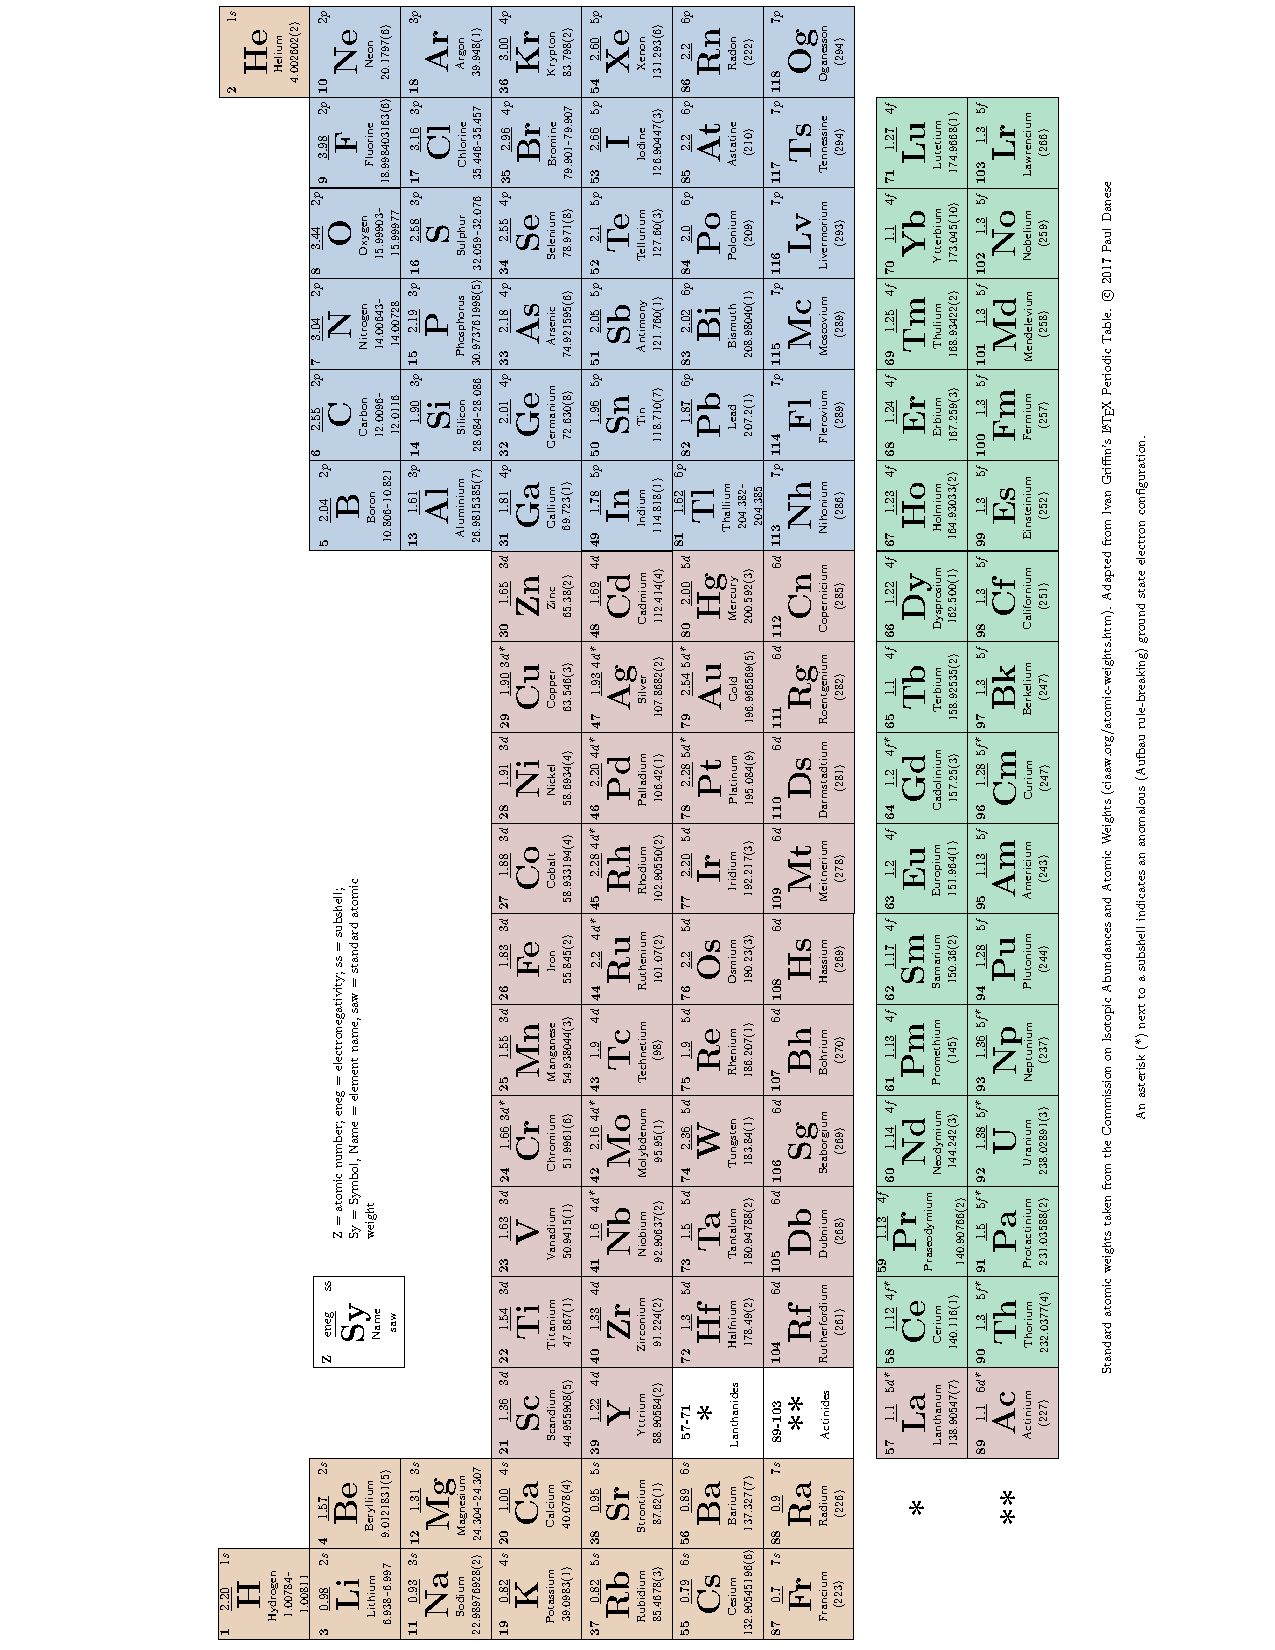
\includepdf[angle=-90,pagecommand={\section{Periodic Table of the Elements}}, scale=0.9]{periodic_table.pdf}

\end{document}
